\chapter{Sumeiden tiivisteiden haasteet\label{fuzzy-problems}}

Sumeat tiivisteet tarjoavat ratkaisun
samankaltaisuutta tarkasteleviin ongelmiin.
Sumeilla tiivisteillä on kuitenkin myös ongelmakohtansa,
joita tässä luvussa käsitellään. Ongelmia ilmenee
sekä yleisellä tasolla että ohjelmistotasolla. Monet
ongelmat vaikuttavat kaikkiin ohjelmistoihin,
mutta ohjelmistoissa ilmenee paikallisiakin puutteita.
Usein nämä ovat virheitä suunnittelussa tai ajan
myötä merkittäviksi kasvaneita puutteita
suorituskyvyssä ja luotettavuudessa.
Sumeita tiivisteitä käytetään haittaohjelmien
torjunnassa, joten niitä vastaan pyritään
luonnollisesti hyökkäämään mitä luovimmin keinoin.

% 4

\section{Rajoitteet}

Sumeat tiivisteet kärsivät suurehkosta määrästä haasteita.
Puutteet eivät kuitenkaan ole helposti kuvattavissa,
vaan monet niistä ilmenevät tilanteesta ja ohjelmistosta
riippuen. Yleisellä tasolla sumeilla tiivisteillä
on rajoitteita, jotka estävät tai hankaloittavat
ohjelmiston optioinnin. Ohjelmistoissa taas
esiintyy ohjelmistokohtaisia puutteita, jotka
ovat korjattavissa.

Keskeinen käytännön rajoite sumeilla tiivisteillä on kyvyttömyys
tulkita syötteiden semantteista merkitystä \textcite{li15}. Nykyiset
sumeat tiivisteohjelmistot tulkitsevat syötteen syntaksitasolla
semanttisten rakenteiden tunnistamisen sijaan. Tämä
mahdollistaa hyökkäykset tiivisteitä vastaan.

Sumeiden tiiviseteiden käyttöä rajoittaa tulosten subjektiivisuus \citep{naik19}.
Kehittyneimmänkään ohjelmiston käsitys samankaltaisuudesta
ei aina vastaa käyttäjän tulkintaa. Samankaltaisuudelle ei voida
määrittää universaalia raja-arvoa ja ohjelmistot ainoastaan
arvioivat samankaltaisuutta niille annettujen sääntöjen mukaisesti.
Eri ohjelmistot voivat tuottaa samalla syötteellä radikaalistikin
poikkeavia tuloksia, joten ohjelmiston valinta on olennaisessa
roolissa. Toisaalta eri tulkitsijat voivat myös tulkita saman
tuloksen eri tavoin. Samanakaltaisuuden määrittämisessä
tiivistysohjelmisto suorittaa ainoastaan kehityksessä
määritetyn havainnoinnin ja jättää tulosten
tulkistemisen ohjelman käyttäjälle.

\begin{figure}
   \centering
   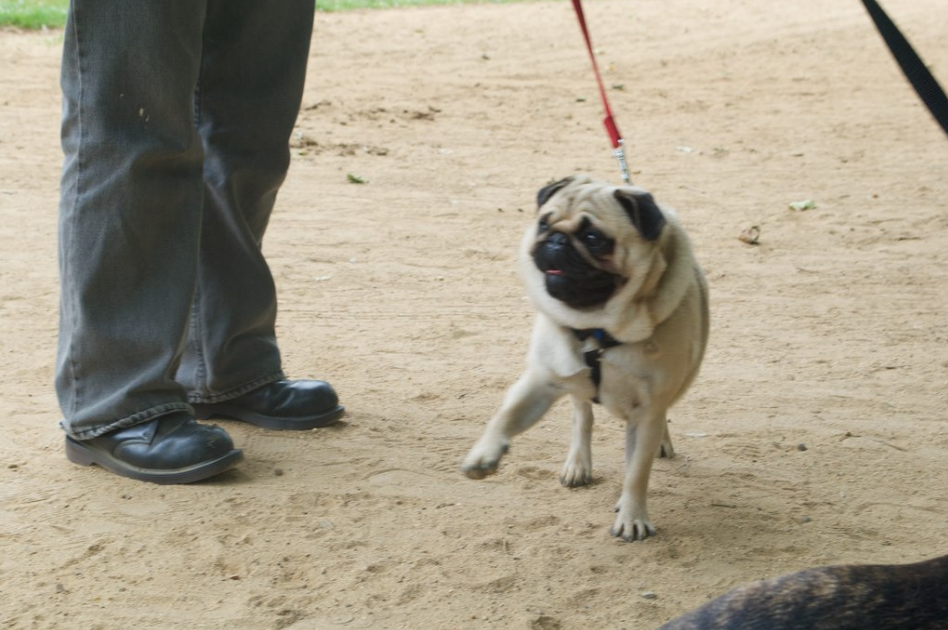
\includegraphics[width=10cm]{../assets/dog-before.png}
   \caption{Naamitoitava kuva}
\end{figure}

\begin{figure}
   \centering
   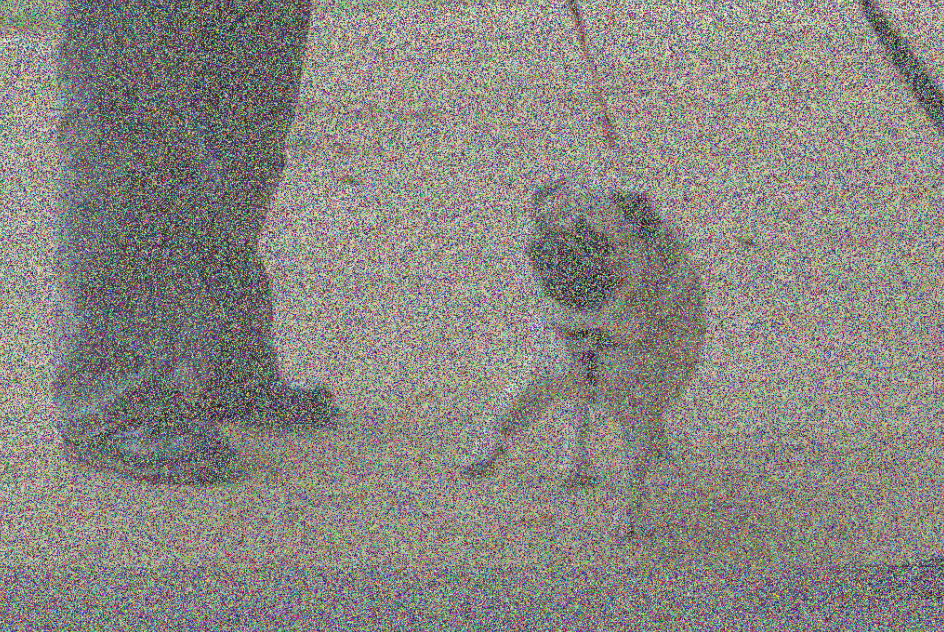
\includegraphics[width=10cm]{../assets/dog-after.png}
   \caption{Ensimmäisessä ja toisessa vaiheessa käsitelty kuva.}
\end{figure}

\section{Puutteet ja haavoittuvuudet}

Sumeita tiivisteitä voidaan yrittää johtaa harhaan eri tavoin. Edellisessä
luvussa käsitellyn haittaohjelman naamioinnin lisäksi menetelmällä, jossa 
harmitonta dataa muokataan tarkoituksellisesti aiheuttamaan osuma jonkin
haitalliseksi todetun sisällön kanssa, voidaan hidastaa haittaohjelmien torjuntaa. 
Haittaohjelmien leviämistä voidaan tehostaa myös kasvattamalla torjuntatyön kuormittavuutta. Kasvanut työmäärä hidastaa haittaohjelmien tunnistamista. Kuormittavuutta voidaan lisätä pyrkimällä aiheuttamaan perättömiä haittaohjelmaepäilyjä. Tällainen
harhautusmahdollisuus on olemassa sumeita tiivisteitä vastaan. \textcite{ermerins} esittää tällaisen uhan erityisesti Ssdeepiä vastaan ja tutkii mahdollisuuksia tulosten vääristelyyn.

\textcite{ermerins} pyrkivät laatimaan menetelmän, jolla olisi mahdollista luoda proseduraalisesti tunnistamattomia kuvia, joiden samankaltaisuus lähdekuvan kanssa olisi suuri. Esitetty menetelmä muokkaa kuvia kahdessa vaiheessa, joista ensimmäisessä luodaan pikseleitä yksitellen muokkaamalla uusi kuva. Tämän kuvan on tarkoitus olla
semanttisesti tunnistamaton, eli ihmisen ei tulisi voida yhdistää niitä
toisiinsa. Edellytyksenä kuitennkin on, että Ssdeep merkitsee osumaksi generoidun kuvan samankaltaiseksi alkuperäisen kanssa. Generoidusta kuvasta luodaan
toisessa vaiheessa nopeasti suuri määrä hieman toisistaan poikkeavia
versioita muuttamalla sattumanvaraisesti valittuja pikseleitä.
Kuvassa 5.1 on tutkimuksessa käytetty alkuperäinen kuva; kuvassa 5.2
on alkuperäisen kuvan käsitelty versio.

Kokeessa havaittiin ssdeep-ohjelmiston kyenneen yhdistämään kaikki generoidut kuvatiedostot alkuperäiseen. Lisäksi generoitujen kuvien huomautetaan olevan ilmeisen
tunnistettavan näköisiä alkkuperäisisen kuvan kanssa. Siten tavoitetta generoida tunnistamattomia kuvatiedostoja ei saavutettu. Lisäksi huomautetaan kehitetyn menetelmän olleen hidas ja sopimaton käytännön sovelluksiin. Tutkimuksessa on esitetty
potentiaalisia optimointikeinoja menetelmän suorituskyvyn kasvattamiseksi.

Datan naamiointia sumeita tiivisteitä vastaan tutkitvat \textcite{oliver14}.
Aiemmin käsitellyn ohjelmien tunnistamisen lisäksi naamiointi suoritettiin
kuva- ja tekstitiedostoille sekä HTML-websivuille käyttäen Ssdeep-, Sdhash-
ja Tlsh-ohjelmistoja. Kuvien naamioinnissa roskapostituksessa
käytettyjä kuvia käännettiin sekä venytettiin, minkä lisäksi
kirjasinkokoa ja -lajia muutettiin. Tekstitiedostoja muutettiin
lisäämällä, poistamalla ja vaihtamalla sanoja, vaihtamalla
rivien paikkaa ja lisäämällä satunnaista dataa. HTML-sivuihin
lisättiin tyhjiä merkkejä sallittuihin kohtiin.

Ssdeepin todetaan suoriutuneen heikoimmin kuvien yhdistämisessä;
Sdhash ja Tlsh suoriutuivat hyvin. Sdhash ei suoriutunut käännettyjen
ja venytettyjen kuvien tunnistamisessa, ja Tlsh tunnisti eniten kuvia.
Tekstitiedostojen muuttaminen aiheutti ongelmia Ssdeepille ja Sdhasille,
Tlsh suoritui paremmin. 500 muokatusta Html-sivuista Ssdeep ja Sdhash
tunnistivat 11 ja 16, ja Tlsh 291. Vertailu osoittaa, että Tlsh suoritui
kaikissa tilanteissa merkittävästi paremmin. Havaitaan, että eri ohjelmistojen
suoriutumisen välillä on merkittäviä eroja, jotka riippuvat syötteen
formaatista. Toiset ohjelmistot reagoivat herkemmin datatyypin
muutokseen tai tarkoitukselliseen harhauttamiseen. Lisäksi
huomautetaan, että erityisesti ohjelmakoodin muuntelu aiheuttaa
em.\ datatyyppejä suuremman haasteen staattiselle
haittaohjelma-analyysille.

\section{Ohjelmistojen erot}

On selvää, että haittaohjelma-analyysissa tutkielmassa käsitelyllyillä
tiivisteohjelmistoilla on mwrkittäviä eroja. Kontekstiriippuvaisten
paloittain määriteltyjen tiivisteiden tunnistuskyky on heikko, ja
Sdhash sekä Mvhash-b vaikuttavat soveltuvan haittaohjelmien tunnistamiseen
paremmin. Erityiseti Ssdeepin ja Sdhashin välillä havaitaan merkittävä
ero tarkkuudessa sekä ohjelmakoodin että muuntyyppisen datan suhteen.

\textcite{martin-perez21} esittävät neljä hyökkäystyyppiä
sumeita tiivisteitä vastaan; samankaltaisuuden vähentäminen
ja simulointi sekä tiivisteiden generoinnin ja vertailun
hankaloittaminen. Hyökkäyksille altistavat tekijät
vaihtelevat, ja suurimmassa osassa ohjelmistoja
esiintyy haavoittuvuuksia. Tutkielmassa
kuvatut ohjelmistot ovat alttiita kaikille
hyökkäystyypeille.

Tietyn ohjelmiston suoriutuminen riippuu suurelta osin tilanteen edellyttämistä
tarpeista ja käsitellyn datan tyypeistä. Sdhashin vahvuuksiin ei kuulu
kokonaisten tiedostojen vertailu, vaan pienempien rakenteiden
havaitseminen \parencite{breitinger12}. Ohjelmistot kärsivät
erilaisista puutteista toteutuksessa.

